% This file was created with tikzplotlib v0.10.1.
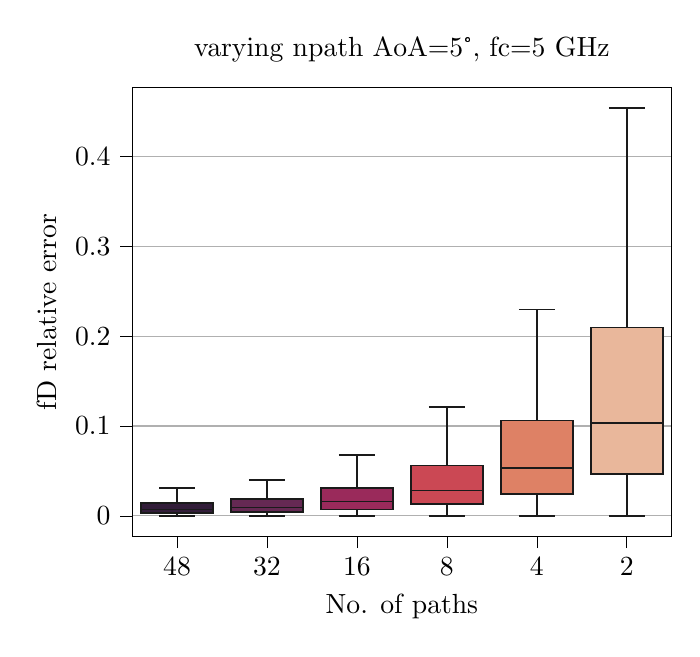
\begin{tikzpicture}

\definecolor{black26}{RGB}{26,26,26}
\definecolor{brown1544291}{RGB}{154,42,91}
\definecolor{burlywood233183155}{RGB}{233,183,155}
\definecolor{darkgray176}{RGB}{176,176,176}
\definecolor{darkslategray1014183}{RGB}{101,41,83}
\definecolor{darkslategray502957}{RGB}{50,29,57}
\definecolor{indianred2037284}{RGB}{203,72,84}
\definecolor{salmon222129101}{RGB}{222,129,101}

\begin{axis}[
tick align=outside,
tick pos=left,
title={varying npath AoA=5°, fc=5 GHz},
x grid style={darkgray176},
xlabel={No. of paths},
xmin=-0.5, xmax=5.5,
xtick style={color=black},
xtick={0,1,2,3,4,5},
xticklabels={48,32,16,8,4,2},
y grid style={darkgray176},
ylabel={fD relative error},
ymajorgrids,
ymin=-0.0226865834736131, ymax=0.476420659195047,
ytick style={color=black}
]
\path [draw=black26, fill=darkslategray502957, semithick]
(axis cs:-0.4,0.00312846566565863)
--(axis cs:0.4,0.00312846566565863)
--(axis cs:0.4,0.0142591336146539)
--(axis cs:-0.4,0.0142591336146539)
--(axis cs:-0.4,0.00312846566565863)
--cycle;
\path [draw=black26, fill=darkslategray1014183, semithick]
(axis cs:0.6,0.00420047635062512)
--(axis cs:1.4,0.00420047635062512)
--(axis cs:1.4,0.0186173518179513)
--(axis cs:0.6,0.0186173518179513)
--(axis cs:0.6,0.00420047635062512)
--cycle;
\path [draw=black26, fill=brown1544291, semithick]
(axis cs:1.6,0.00722352357152707)
--(axis cs:2.4,0.00722352357152707)
--(axis cs:2.4,0.031286936446514)
--(axis cs:1.6,0.031286936446514)
--(axis cs:1.6,0.00722352357152707)
--cycle;
\path [draw=black26, fill=indianred2037284, semithick]
(axis cs:2.6,0.0129013520154952)
--(axis cs:3.4,0.0129013520154952)
--(axis cs:3.4,0.0561329628902816)
--(axis cs:2.6,0.0561329628902816)
--(axis cs:2.6,0.0129013520154952)
--cycle;
\path [draw=black26, fill=salmon222129101, semithick]
(axis cs:3.6,0.0239714148776893)
--(axis cs:4.4,0.0239714148776893)
--(axis cs:4.4,0.10624069653294)
--(axis cs:3.6,0.10624069653294)
--(axis cs:3.6,0.0239714148776893)
--cycle;
\path [draw=black26, fill=burlywood233183155, semithick]
(axis cs:4.6,0.0468841206163041)
--(axis cs:5.4,0.0468841206163041)
--(axis cs:5.4,0.209633887848842)
--(axis cs:4.6,0.209633887848842)
--(axis cs:4.6,0.0468841206163041)
--cycle;
\addplot [semithick, black26]
table {%
0 0.00312846566565863
0 1.09374962390471e-07
};
\addplot [semithick, black26]
table {%
0 0.0142591336146539
0 0.0309547513011629
};
\addplot [semithick, black26]
table {%
-0.2 1.09374962390471e-07
0.2 1.09374962390471e-07
};
\addplot [semithick, black26]
table {%
-0.2 0.0309547513011629
0.2 0.0309547513011629
};
\addplot [semithick, black26]
table {%
1 0.00420047635062512
1 7.36455465382756e-07
};
\addplot [semithick, black26]
table {%
1 0.0186173518179513
1 0.0402411863058504
};
\addplot [semithick, black26]
table {%
0.8 7.36455465382756e-07
1.2 7.36455465382756e-07
};
\addplot [semithick, black26]
table {%
0.8 0.0402411863058504
1.2 0.0402411863058504
};
\addplot [semithick, black26]
table {%
2 0.00722352357152707
2 1.33307940903596e-07
};
\addplot [semithick, black26]
table {%
2 0.031286936446514
2 0.0673656637471981
};
\addplot [semithick, black26]
table {%
1.8 1.33307940903596e-07
2.2 1.33307940903596e-07
};
\addplot [semithick, black26]
table {%
1.8 0.0673656637471981
2.2 0.0673656637471981
};
\addplot [semithick, black26]
table {%
3 0.0129013520154952
3 1.50820755208037e-07
};
\addplot [semithick, black26]
table {%
3 0.0561329628902816
3 0.120945876122493
};
\addplot [semithick, black26]
table {%
2.8 1.50820755208037e-07
3.2 1.50820755208037e-07
};
\addplot [semithick, black26]
table {%
2.8 0.120945876122493
3.2 0.120945876122493
};
\addplot [semithick, black26]
table {%
4 0.0239714148776893
4 1.78757409160517e-07
};
\addplot [semithick, black26]
table {%
4 0.10624069653294
4 0.229637870601489
};
\addplot [semithick, black26]
table {%
3.8 1.78757409160517e-07
4.2 1.78757409160517e-07
};
\addplot [semithick, black26]
table {%
3.8 0.229637870601489
4.2 0.229637870601489
};
\addplot [semithick, black26]
table {%
5 0.0468841206163041
5 3.34381426203771e-06
};
\addplot [semithick, black26]
table {%
5 0.209633887848842
5 0.453733966346472
};
\addplot [semithick, black26]
table {%
4.8 3.34381426203771e-06
5.2 3.34381426203771e-06
};
\addplot [semithick, black26]
table {%
4.8 0.453733966346472
5.2 0.453733966346472
};
\addplot [semithick, black26]
table {%
-0.4 0.00706678204608885
0.4 0.00706678204608885
};
\addplot [semithick, black26]
table {%
0.6 0.0093840675592792
1.4 0.0093840675592792
};
\addplot [semithick, black26]
table {%
1.6 0.0159837043700747
2.4 0.0159837043700747
};
\addplot [semithick, black26]
table {%
2.6 0.0283702440329193
3.4 0.0283702440329193
};
\addplot [semithick, black26]
table {%
3.6 0.0533822375891471
4.4 0.0533822375891471
};
\addplot [semithick, black26]
table {%
4.6 0.103396997703011
5.4 0.103396997703011
};
\end{axis}

\end{tikzpicture}
